\clearpage
\section{Practical part}

%%%%%%%%%%%%%%%%%%%%%%%%%%%%%%%%%%%%%%%%

\subsection{Starting from the H2b baseline code}
We provide you again with a baseline project already present inthe \texttt{mcu} folder of the git. Do not forget to syncrhonize your git before starting the Hands-On. The baseline code is almost the same as the H2a baseline code, except the interrupt line for the button that has been activated and a few functions for formatting the prints. Import and open the project as explained in the previous Hands-On and flash it on your MCU. The LED2 should be blinking. We will build onto this project.

%%%%%%%%%%%%%%%%%%%%%%%%%%%%%%%%%%%%%%%%

\subsection{Adding a new peripheral: bring the ADC in the project!}
Our microphone/mini-jack input is connected to pin \textbf{PA0}. Open the \texttt{.ioc} file, go to \textbf{Analog} in the left bar menu, select the \textbf{ADC1} peripheral, select input 5 (IN5) as \textbf{IN5 Single-ended}, which correspond to the \textbf{PA0} pin set to \textbf{ADC1\_IN5}. Activating the ADC creates an error by default in its clock configuration, to correct this, open the \textbf{Clock configuration} tab. You will be prompted to resolve automatically the errors, although it might work sometimes, in this case, it will alter the main clock speed, which we want to avoid : click on \textbf{No} to solve the error manually. The errors are highlighted in magenta as you can see in \autoref{fig:adc_clock_tree}. Choose \textbf{SYSCLK} as clock source for the ADC to solve the problem, you don't need to modify anything else.

\begin{figure}[h]
    \centering
    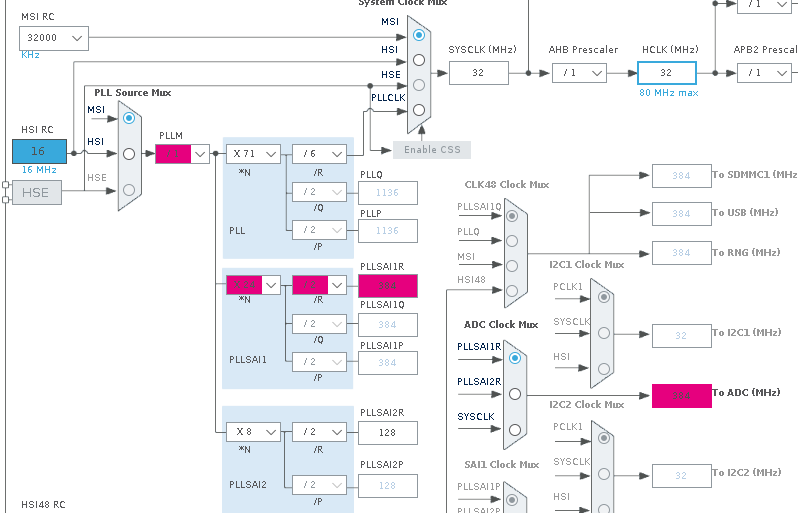
\includegraphics[scale=0.4]{figures/adc_clock_tree.png}
    \caption{ADC clock tree configuration error. }
    \label{fig:adc_clock_tree}
\end{figure}

For a basic usage of the ADC, that's all there is to it. We advise you to take a look at the manuals available on Moodle to understand the purpose of all the parameters of the ADC. You can now save and regenerate the code.\\

\noindent To be able to read a value of the ADC, you need to use the following three functions :
\begin{enumerate}
    \item \texttt{HAL\_ADC\_Start(\&hadc1)} to prepare the ADC.
    \item \texttt{HAL\_ADC\_PollForConversion(\&hadc1,0xFFFF)} triggers the ADC conversion and stores the value in the register of the ADC. The second argument of the function corresponds to the timeout in seconds for the conversion. This function returns a \texttt{HAL\_OK} value if the conversion went well or a \texttt{HAL\_ERROR} in case of error.
    \item \texttt{HAL\_ADC\_GetValue(\&hadc1)} retrieves the value from the ADC and returns it. It is good practice to call this function inside an \texttt{if} condition, only when the previous function returned no errors. The returned type is an \texttt{uint32\_t} unsigned int.
    \item \texttt{HAL\_ADC\_Stop(\&hadc1)} to stop the acquisition.
 \end{enumerate}

\noindent Write a program where you return the sample once the value of the \textbf{PA0} pin every time we press the user button. It will be hard to test your code with sound: we therefore recommend to use your ADALM2000 to generate a DC signal. Connect it to \textbf{pin 2} of the \textbf{SEL\_SOUND} header (you will need to remove the jumper: do not lose it!). Note: a simpler, while functional setup to test your code could be to connect the \textbf{pin 2} of the \textbf{SEL\_SOUND} header to either VDD or GND, which avoids the need to use the ADALM2000 (but restrains you to only two values). We provide you again with a python script to read the data coming from the MCU to your computer. To do so, run the \texttt{basic-uart-reader.py} script.\\
\begin{bclogo}[couleur = gray!20, arrondi = 0.2, logo=\bcattention]{Absolute maximum ratings}
The MCU is a sensitive device, it is not designed to handle any kind of voltage on its pins. Take a look at Section 6.2 of the MCU datasheet, you can find here that the maximum voltage on a pin cannot be higher than 4 volts. The ADALM2000 can go beyond that, pay attention to never go above this value, it is recommended to stay below \textbf{VDD}: 3.3V.
\end{bclogo}
\begin{bclogo}[couleur = gray!20, arrondi = 0.2, logo=\bcquestion]{Digitized values}
Take a look at the values given by your ADC. How many possible values are possible? How many bits are used for the quantization?
\end{bclogo}

\begin{bclogo}[couleur = gray!20, arrondi = 0.2, logo=\bcquestion]{Reading a schematic}
How do we know that the microphone/mini-jack input is connected to the pin \textbf{PA0} ? \textbf{Hint}: use the schematic of the custom board provided in the \texttt{Guide - how to use the boards.pdf} and the schematic of the Nucleo MCU board. Both are available in the \texttt{Technical ressources} folder on Moodle.
\end{bclogo}

%%%%%%%%%%%%%%%%%%%%%%%%%%%%%%%%%%%%%%%%

\subsection{Advanced management of audio acquisition: using ADC, DMA and a TIMER}

\noindent As our ultimate goal is to be able to sample an audio signal, we must have a steady sampling at a defined frequency (in order not to introduce distortion in the signal and to make sure Nyquist criterion is fulfilled). To do this, we will use a TIMER. However, this time we won't link the timer to a external pin but an internal signal. Similarly, we won't use C code to trigger an ADC conversion but rather use the signal of the timer. Finally, we won't use C code either to retrieve the ADC value, but rather set up the DMA to copy directly to an array in memory that will be accessed by the C code. The \textbf{DMA} (Direct Memory Access) is a new peripheral that we will have to introduce in this project. Its purpose is to transfer data from one address to an other one, without using the CPU to perform this action. This allows more advanced sampling and lower power consumption as we do not need the CPU to be running and awake. In this project, the life of one sample starts by the timer triggering an ADC conversion. Then when the conversion is done, the ADC will trigger the DMA to transfer the sample to the correct address. \\

\noindent We will start by setting up the timer TIM3, open this peripheral in the \texttt{.ioc} file. Set the \textbf{Clock source} as \textbf{Internal clock} to activate the timer. Our sampling frequency will be 11kHz, so as our clock is set 32MHz, we will use 15 as prescaler and 195 as period values. This will provide a timer frequency of just under 11kHz, i.e., 10.2 kHz. Next, we need to set up the periodic signal that will trigger the ADC. To do so, open the parameters of the TIMER and in the bottom panel under \textbf{Trigger Output (TRGO) Parameters} , choose \textbf{Update event} for \textbf{Trigger event selection (TRGO)}. \\

\noindent Here are key settings that you must set to ensure that the ADC and the DMA are working as we expect :
\begin{itemize}
    \item In the ADC parameters, we need to reconfigure the trigger source to the timer. Follow \textbf{ADC regular conversion mode} $\rightarrow$ \textbf{External trigger conversion source} $\rightarrow$ \textbf{Timer 3 trigger out event}.
    \item Now, we need to configure the DMA, head into the DMA tab. Click on \textbf{Add}. In DMA request, you can choose ADC1. The rest can be left at the default value. Notice that the mode of the DMA is set to "Normal".
    \item Note that we don't need to make sure that the DMA will be able to tell us when the sampling is finished as it's interrupt is enabled by default and cannot be disabled. You can see this in the NVIC tab.
    %\item Parameter settings tab -> ADC settings -> DMA continuous requests -> Enabled
    %\item Code : timer start, ADC start, set up interrupt handlers
\end{itemize}
\noindent Now, save the \texttt{.ioc} file and regenerate the code. You will have to call the following 2 functions to launch the sampling :
\begin{itemize}
    \item \texttt{HAL\_TIM\_Base\_Start(\&htim3)} : to start the timer. Note that this function is different from the one used in the last hands-on. We don't need to use an output compare channel so the base of the timer is needed only.
    \item \texttt{HAL\_ADC\_Start\_DMA(\&hadc1, (uint32\_t *)ADCBuffer, ADC\_BUF\_SIZE)} : to start the sampling. It will sample ADC\_BUF\_SIZE samples at the ADCBuffer pointer. It will trigger an interrupt when the transfer is complete.
    \item To stop the sampling, you can use \texttt{HAL\_TIM\_Base\_Stop(\&htim3)} and \texttt{HAL\_ADC\_Stop\_DMA(\&hadc1)}.
    \item \texttt{void HAL\_ADC\_ConvCpltCallback(ADC\_HandleTypeDef *hadc)} : is the callback function of the complete DMA transfer.
\end{itemize}

\noindent We ask you to implement the following functionality : On the push of a button, start sampling and fill up the buffer ADCBuffer with 256 samples. Then at the end of the sampling, print the data to the UART as the next section describes it. In order to test the functionality of your code, generate a pure sine at 1 kHz on the \textbf{pin 2} of the \textbf{SEL\_SOUND} header which is connected to the \textbf{PA0} pin. This can be done by using the ADALM2000 in AWG (Arbitrary Waveform Generator) mode. Launch the script and observe the plot generated. Check if your sampling speed is correct.


%%%%%%%%%%%%%%%%%%%%%%%%%%%%%%%%%%%%%%%%


\subsection{Getting the data out of the MCU and post-process it on Python}

Now that you have your data acquired and stored on you MCU, you need to get it out to make sure it worked properly. As already sketched in the H2a, you can do this by using the UART interface. It is easy to read a few values in the terminal but this becomes really more difficult when dealing with thousands of samples. For that reason, we provide you a Python script that will parse the UART data into something easily understandable by humans. This section explains how to format your data on the MCU side such that the script will read it correctly. The code provided is a baseline: feel free to reuse it to improve and extend the functionalities !

\subsection*{On the MCU side: formatting the data}
First, take a bit of time to understand the few lines of code in the \texttt{main.c} file. Their purpose is to format the data that we will send to the computer. As you can notice in the code, we will encode your audio buffer in a single block of hexadecimal values.

\begin{lstlisting}[columns=fullflexible]
void hex_encode(char* s, const uint8_t* buf, size_t len) {
    s[2*len] = '\0'; // A string terminated by a zero char.
    for (size_t i=0; i<len; i++) {
        s[i*2] = "0123456789abcdef"[buf[i] >> 4];
        s[i*2+1] = "0123456789abcdef"[buf[i] & 0xF];
    }
}

void print_buffer(uint16_t *buffer) {
	hex_encode(hex_encoded_buffer, (uint8_t*)buffer, sizeof(buffer));
	printf("SND:HEX:%s\r\n", hex_encoded_buffer);
}
\end{lstlisting}
%\begin{bclogo}[couleur = gray!20, arrondi = 0.2, logo=\bcquestion]{Paying attention to types when programming}
%In the first block of code, can you explain why we use the factor 4 for indexing ? Make sure the hexadecimal encoding function is clear for you.
%\end{bclogo}

\begin{bclogo}[couleur = gray!20, arrondi = 0.2, logo=\bcinfo]{Parsing prefix}
In the second block of code, have you noticed the \texttt{"SND:HEX:"} prefix ? This is important to make sure it is written exactly that way. It is indeed used in the Python script as a parsing prefix.
\end{bclogo}

\noindent To make sure it is working properly, you can now save, compile and flash your code on the MCU. Run the \texttt{basic-uart-reader.py} script and check out that it is behaving as expected !

\subsection*{On the computer side: Python script to post-process your data}

Then, you need to handle the data coming from the UART interface in a controlled way and with more details than the basic python script. This is the purpose of the \texttt{uart-reader.py} that we provided you. Before running the script in the terminal, we expect you to dive into it to avoid the "black box effect" which prevents a good understanding of what is going on.

\begin{bclogo}[couleur = gray!20, arrondi = 0.2, logo=\bcattention]{Launching a python script with uv}
This new script \texttt{uart-reader.py} makes use of different python libraries, as will do many other scripts in this project. It is thus mandatory to run it with uv, with \texttt{uv sync} then \texttt{uv run python <script>}.
\end{bclogo}

\begin{bclogo}[couleur = gray!20, arrondi = 0.2, logo=\bcquestion]{Handling data in the UART interface}
Did you understand how the script manages to handle new data coming from UART, even if it is popping at an unexpected time ? How does the script handle data which does not start with the \texttt{"SND:HEX:"} prefix ? \\

\noindent How are "packets" of data separated?
\end{bclogo}

\noindent When you have understood the script, you can create a new folder called \texttt{audio\_files} in the same directory. It is now time to run it in the terminal by using the command \texttt{python3 uart-reader.py}. It will run until you press on \texttt{Ctrl+C}. Each time new data is coming from the UART, you should see a Figure plotting the data that has been received and an audio file should be generated in the \texttt{audio\_files} folder. The file format (\texttt{.ogg}) is the same as the one of the database you discovered during the first week. If everything worked as expected, you should see your sine wave and even be able to listen to the corresponding audio file.

%%%%%%%%%%%%%%%%%%%%%%%%%%%%%%%%%%%%%%%%

\subsection{Implementing a double buffering approach in your system}
What happens if we want to sample audio continuously? We will have to tweak a bit our peripherals but it's not complicated. In order to sample continuously, we need two buffers, one that we use for sampling, and an other one for processing the data. When we finish sampling into one buffer, we process it and continue sampling into the other one. This technique is called double buffering and is illustrated in \autoref{fig:double_buff}. In the STM platform, we won't exactly have two buffers but one big buffer cut in halves. The DMA actually triggers interrupts not only when the transfer is finished but also when half the transfer is complete. The callback for the half complete transfer is \texttt{void HAL\_ADC\_ConvHalfCpltCallback} and it works exactly the same way as the transfer complete callback.\\

\begin{figure}[h]
    \centering
    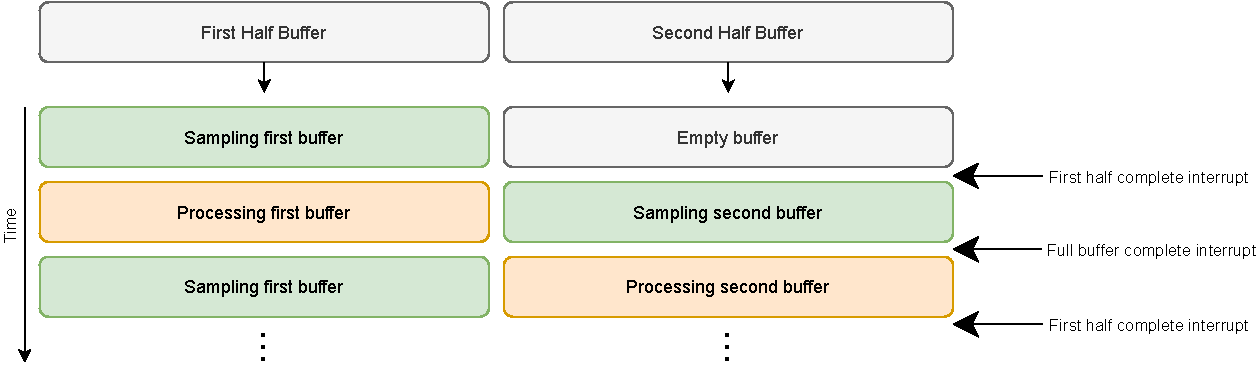
\includegraphics[scale=0.8]{figures/double_buffering.pdf}
    \caption{Illustration of the double buffering technique}
    \label{fig:double_buff}
\end{figure}

\noindent The parameters we need to change in our peripherals are the following :
\begin{itemize}
    \item Open the parameters of the \textbf{DMA} and select the line corresponding to \textbf{ADC1}. Change the mode to \textbf{circular}. This will result in the DMA automatically setting its destination address back to the initial address whenever it reaches the end address. If we did not set the mode to circular, the DMA would continue incrementing the destination address and would reach an undesired address space.
    \item We also must tell the ADC to not stop triggering the DMA when it reaches the desired amount of samples. We do this by opening the \textbf{ADC1} parameters, then enable \textbf{ADC\_Settings} $\rightarrow$ \textbf{DMA Continuous Requests}.
\end{itemize}

%In the previous example, you might have noticed that you only used the half of the buffer available for ADC data. This is normal as you explicitly stopped the acquisition in the callback when half of the buffer is full, i.e., \texttt{void HAL\_ADC\_ConvHalfCpltCallback}. We will now introduce you to a well-known technique called the \textit{double buffering}. The concept is simple but powerful: by splitting a buffer in two parts (fixed in advance), you can acquire data on one part of the buffer while working on the other one with the CPU. This allows you to perform audio acquisition continuously, without blind spot (in theory!). It is crucial do be careful to avoid mixing up everything and polluting your acquisition. Thanks to the two IRQs sent by the DMA when it reaches a half buffer or a full buffer, we can handle this in a nice way in the respective callbacks. \\

\noindent In the C code, when you call the \texttt{HAL\_ADC\_Start\_DMA} function, make sure to adjust the sampling size by doubling it. The \texttt{ADCBuffer} array is already sized for double buffering. You can also access easily the first or second buffer thanks to the \texttt{ADCData1} and \texttt{ADCData2} pointers.\\

\noindent With this, the double buffering technique is ready. We expect you to program the following functionality : When you press on the button, the ADC starts in a double buffering mode, for each half buffer, calculate the power contained in the digitized signal and print its value to the UART stream, if it exceeds a threshold value of 50\footnote{This value was choosen using the mini-jack cable, you might need to update this value if you use the microphone based on the ambient noise.}, you sample one more buffer, stop the sampling and send the data through the same way as before. Use the script detailled in the previous section to save your audio files. You can adjust the buffer size easily on the MCU with the \textbf{ADC\_BUF\_SIZE} constant which corresponds to the number of samples. You can safely go up to 30000 samples($\approx$3 seconds). Finally, don't worry, the UART transfer might take several seconds to process. \\

\noindent The function to calculate the signal power is the following : \texttt{get\_signal\_power(uint16\_t *buffer, size\_t len)}.


\begin{bclogo}[couleur = gray!20, arrondi = 0.2, logo=\bcquestion]{Hardware constraints}
In this example, we asked you to acquire data during 3 seconds. Obviously, the quantity of data that it represents depends directly on the sampling frequency and the total size also depends on the type chosen for each sample. When you are programming on your computer, you usually are not limited to such small amounts of data of constraints as you have massive amount of memory available. This is not true anymore when dealing with embedded programming as the hardware you are using is a way more constrained.
\begin{itemize}
    \item In your system, what is the amount of memory available (flash and RAM)?
    \item Given the type chosen for your ADC samples, what is a good approximation of the theoretical maximal size of your buffer? You can find this information in the datasheet of the MCU.
    \item What are the trade-offs between sampling frequency, resolution and hardware requirements?
    \item Would we be able to send all the samples directly onto the UART stream with the current baudrate of 115200?
    \item What is the limit of the ADC buffer size in samples and what limits it?
\end{itemize}

\end{bclogo}

\noindent Check out the signal sampled by the ADC when you chose the microphone or the mini-jack as audio source on the custom board (please refer to the \texttt{Guide - how to use the boards.pdf} in the folder \texttt{Technical ressources} on Moodle before doing any changes on the custom board). Does it seems coherent when you compare it (visually) to the signal observed on an oscilloscope ?

\begin{bclogo}[couleur = gray!20, arrondi = 0.2, logo=\bcquestion]{Sampling frequency and Nyquist criterion}
As the hardware is set on your custom board (fixed values for resistance, capacitors, ...), how does it constrain you regarding the minimal sampling frequency needed by your system ? Where can you find the information for the custom board ? What is the main difference between the output of the AFE and the output of the mini-jack regarding these considerations ? \\

\noindent How can the ADC be impacted when changing the frequency clock of the system ? Why is it critical to be aware of that ?
\end{bclogo}
%%%%%%%%%%%%%%%%%%%%%%%%%%%%%%%%%%%%%%%%
